\clearpage

\section{Simulation Analysis}
\label{sec:simulation}

The circuit, as is presented on Figure \ref{fig:circuit}, was simulated using \textit{NGSpice}.

\vspace{-0.2cm}

\subsection{Voltage Gain}

We first took a look at what happened in node \textit{out} compared to node \textit{in2}, which suffered the effect from both of the stages of the circuit, using frequency analysis. The result is presented in Figure \ref{fig:sim-gain}.

\vspace{-3cm}

\begin{figure}[h] \centering
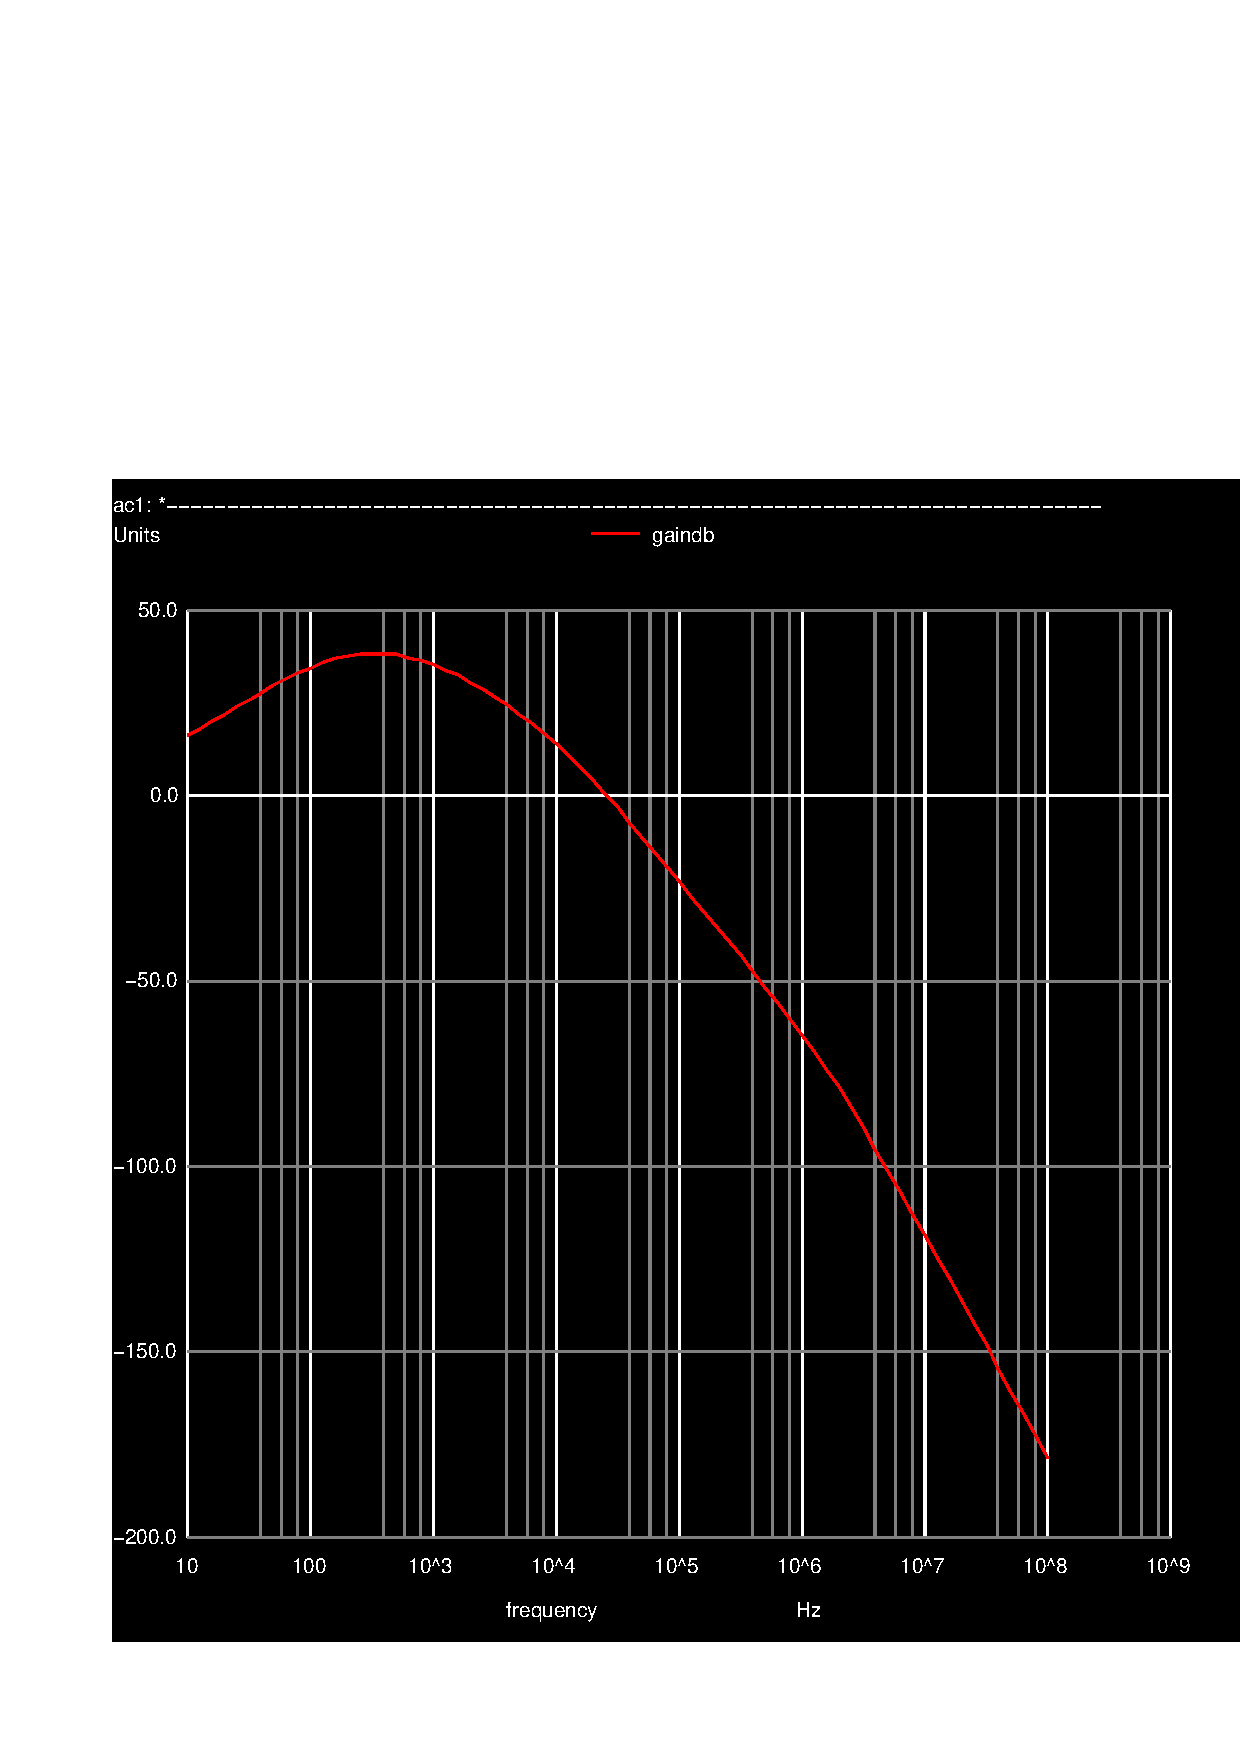
\includegraphics[width=0.5\linewidth]{../sim/gain.pdf}
\caption{Output Voltage Gain Simulated}
\label{fig:sim-gain}
\end{figure}

This graph is the consequence of a passband filter, which means that there is only a specific set of values - a band, if you will - where the circuit works the way it is supposed to. In this case, the passband filter works between around $10^4$ and $10^6$ Hz, which means the amplifier barely works for the human ear.

The value for the highest point in the graoh is shown below.

\vspace{0.4cm}

\begin{center}
\begin{tabular}{|l|r|}
  \hline    
  {\bf Variable} & {\bf Value (dB)} \\ \hline
  gaindbmax & 3.834218e+01\\ \hline

\end{tabular}
\end{center}

\vspace{0.4cm}

Additionaly, we worked out the bandwidth, which is shown below.

\vspace{0.4cm}

\begin{center}
\begin{tabular}{|l|r|}
  \hline    
  {\bf Variable} & {\bf Value} \\ \hline
  \input{../sim/bandwidth_tab.tex}
\end{tabular}
\end{center}

\vspace{0.4cm}

The value of the bandwidth shows for how long the passband filter works - i.e. for how much of the frequencies tested the circuit actually amplifies.


\newpage
\subsection{Input and Output Impedances}

To work out the input impedance, we simply measured the voltage in node \textit{in2}, the node of the input stage of the circuit, and divided it by the current going through it. The result is shown in the table below, with the first value being the real part and the second value being the imaginary part.

\vspace{0.4cm}

\begin{center}
\begin{tabular}{|l|r|}
  \hline    
  {\bf Variable} & {\bf Value ($k\Omega$)} \\ \hline
  zin & 9.999982e+02,-3.99820e+02\\ \hline

\end{tabular}
\end{center}

\vspace{0.4cm}

For measuring the output impedance, we had to change the circuit used in \textit{NGSpice}. We turned off source $V_{in}$, leaving it in short circuit. Furthermore, we substituted the load, which was the component that was overseeing the whole circuit, with a dummy voltage source equal to the one we turned of, calling it $V_L$ as it is in the place of the load. This circuit can be observed in Figure \ref{fig:circuit-2-spice}.

\vspace{0.4cm}


\begin{figure}[h] \centering
\includegraphics[width=0.6\linewidth]{circuit-with-node-names-out.pdf}
\caption{Circuit used for measuring the output impedance.}
\label{fig:circuit-2-spice}
\end{figure}

\vspace{0.4cm}

The final result of the output load is seen is below, dividing the values we got for the voltage in node \textit{out} and dividing it through the current going through it.

\vspace{0.4cm}

\begin{center}
\begin{tabular}{|l|r|}
  \hline    
  {\bf Variable} & {\bf Value ($k\Omega$)} \\ \hline
  zout & 8.011868e+02,-3.99270e+02\\ \hline

\end{tabular}
\end{center}

\vspace{0.4cm}



\subsection{Merit}

Lastly, we calculated the merit, which is shown below.

\vspace{0.4cm}

\begin{center}
\begin{tabular}{|l|r|}
  \hline    
  {\bf Variable} & {\bf Value} \\ \hline
  merit & 5.223670e-02\\ \hline

\end{tabular}
\end{center}